\section{Rectification}

\begin{frame}
    \begin{itemize}
        \item Ajouter une continuation aux paramètres de la fonction
        \item Remplacer les appels récursifs non terminaux par un appel récursif
              avec une nouvelle continuation
        \item Remplacer les retours de fonction par des appels à la continuation
    \end{itemize}
\end{frame}

\subsection{Ensembles rectifiants}

\begin{frame}[fragile,t]
    \frametitle{Ensembles rectifiants}

    \begin{itemize}
        \item Un \important{ensemble rectifiant} pour une fonction donnée est un
              ensemble d'identifiants susceptibles de mener à un appel
              récursif.
    \end{itemize}

    \vspace{0.2cm}

    \pause

    \begin{minipage}[t]{0.5\textwidth}
        \small \begin{minted}{ocaml}
let rec sum l =
    match l with
    | [] -> 0
    | x :: q -> x + sum q
        \end{minted}

        \uncover<3->{
            \begin{tikzpicture}[remember picture,overlay]
                \draw[red,thick,rounded corners] ([yshift=13,xshift=130]pic cs:start) rectangle ([yshift=26,xshift=160]pic cs:stop);
            \end{tikzpicture}
            $$E = \{ \texttt{sum} \}$$
        }
    \end{minipage}%
    \begin{minipage}[t]{0.5\textwidth}
        \vspace{-0.8cm}
        \small \begin{align*}
            a_1 :=\  & \texttt{l}                                          \\
            a_2 :=\  & \texttt{match } a_1 \texttt{ with}                  \\
                     & \texttt{| [] -> } \begin{aligned}[t]
                                             a_3 & := 0
                                         \end{aligned}                 \\
                     & \texttt{| x :: q -> } \begin{aligned}[t]
                                                 a_4 & := \texttt{x}           \\
                                                 a_5 & := \texttt{sum}         \\
                                                 a_6 & := \texttt{q}           \\
                                                 a_7 & := a_5 \ a_6            \\
                                                 a_8 & := a_4 \texttt{ + } a_7
                                             \end{aligned}
        \end{align*}

        \uncover<4->{
            \begin{tikzpicture}[remember picture,overlay]
                \draw[red,thick,rounded corners] ([yshift=25,xshift=120]pic cs:start) rectangle ([yshift=38,xshift=145]pic cs:stop);
            \end{tikzpicture}
            $$E = \{ \texttt{sum}, a_5 \}$$
        }
    \end{minipage}
\end{frame}

\begin{frame}
    \frametitle{Optimisation des ensembles rectifiants}

    ENS\_RECTIFIANT :
    \vspace{-0.3cm}
    $$
        \left \{ \begin{tabular}{@{}l@{}c@{}l}
            \textbf{Entrée}
             & \textbf{ : }
             & l une forme linéaire, $k \in \mathbb{N}$
            \\ \text{\textbf{Sortie}}
             & \textbf{ : }
             & Existe-t-il un ensemble $E$ rectifiant $l$ tel que $|E| \leq k$?
        \end{tabular} \right .
    $$

    \vspace{0.5cm}
    \pause

    \begin{itemize}
        \item ENS\_RECTIFIANT est \important{indécidable}.
              \pause
        \item Notre algorithme ne marchera pas dans tous les cas possibles.
    \end{itemize}
\end{frame}

\subsection{Rectification}

\begin{frame}[fragile]
    \frametitle{Rectification}

    \RestyleAlgo{plain}
    \tiny \begin{algorithm}[H]
        \Input{Une forme linéaire $l$ rectifiée par $E$}
        \Output{Une forme linéaire correcte $l'$ récursive terminale}

        \vspace{0.2cm}

        $(a, e) \leftarrow$ le premier élément de $l$ \\
        $q \leftarrow$ le reste de $l$ \\

        \uSi{$e$ ne contient pas d'appel à une fonction de $E$}{
            \uSi{$q$ est vide}{
                Renvoyer $\begin{aligned}
                        a   & := e                & \\
                        res & := \texttt{cont } a &
                    \end{aligned}$
            }\uSinon{
                $q_{rec} \leftarrow$ Rectifier($q$, $E$) \\
                Renvoyer $[(a, e)].q_{rec}$
            }
        }\uSinon{
            \uSi{$e$ est un appel de fonction}{
                $e_{rec} \leftarrow$ $e$ avec \texttt{cont} rajouté en dernier
                argument
            }\uSinon{
                $e_{rec} \leftarrow$ $e$ avec chaque enfant localement terminal $c$
                remplacé par Rectifier($c$, $E$)
            }

            \bigskip

            \uSi{$q$ est vide}{
                Renvoyer $[(a, e_{rec})]$
            }\uSinon{
                $q_{rec} \leftarrow$ Rectifier($q$, $E$) \\
                Renvoyer $\begin{aligned}
                        \texttt{new\_cont} & := \texttt{fun } a \texttt{ -> } q_{rec} & \\
                        \texttt{cont}      & := \texttt{new\_cont}                    & \\
                        a                  & := e_{rec}                               &
                    \end{aligned}$
            }
        }
    \end{algorithm}

    \begin{tikzpicture}[remember picture,overlay]
        \draw<2>[mauve,thick,rounded corners] ([yshift=0,xshift=30]pic cs:start) rectangle ([yshift=40,xshift=145]pic cs:stop);
        \draw<3>[mauve,thick,rounded corners] ([yshift=84,xshift=30]pic cs:start) rectangle ([yshift=91,xshift=167]pic cs:stop);
        \draw<4>[mauve,thick,rounded corners] ([yshift=125,xshift=30]pic cs:start) rectangle ([yshift=144,xshift=105]pic cs:stop);
    \end{tikzpicture}
\end{frame}

\begin{frame}[fragile]
    \frametitle{Application}

    \begin{adjustwidth}{-1.5em}{-1.5em}

        \small \begin{minted}{ocaml}
let rec sum (l : int list) : int =
    match l with
    | [] -> 0
    | x :: q -> x + sum q
        \end{minted}

        \vspace{0.2cm}
        \begin{center}
            $\Big\downarrow$
        \end{center}
        \vspace{0.2cm}

        \small \begin{minted}{ocaml}
let rec sum (l : int list) (cont : int -> 'ret) : 'ret =
    match l with
    | [] -> cont 0
    | x :: q ->
        let new_cont (a_7 : int) : 'ret = cont (x + a_7) in
        sum q new_cont

let s = sum [0; 1; 2] (fun res -> res)
        \end{minted}

    \end{adjustwidth}
\end{frame}

\subsection{Accumulateurs}

\begin{frame}[t]
    \frametitle{Accumulateurs}

    \begin{center}
        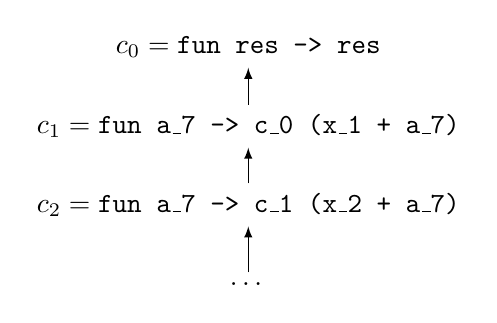
\begin{tikzpicture}
            \node<1-> (c0) at (0, 0) {$c_0 = \texttt{fun res -> res}$};

            \node<2-> (c1) at (0, -1) {$c_1 = \texttt{fun a\_7 -> c\_0 (x\_1 + a\_7)}$};
            \draw<2->[-latex] (c1.north) to (c0.south);

            \node<3-> (c2) at (0, -2) {$c_2 = \texttt{fun a\_7 -> c\_1 (x\_2 + a\_7)}$};
            \draw<3->[-latex] (c2.north) to (c1.south);

            \node<4-> (c3) at (0, -3) {\ldots};
            \draw<4->[-latex] (c3.north) to (c2.south);
        \end{tikzpicture}
    \end{center}
\end{frame}

\addtocounter{framenumber}{-1}
\begin{frame}[t]
    \frametitle{Accumulateurs}

    \begin{center}
        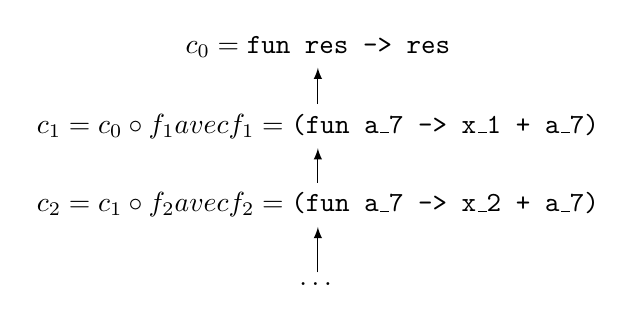
\begin{tikzpicture}
            \node (c0) at (0, 0) {$c_0 = \texttt{fun res -> res}$};

            \node (c1) at (0, -1) {$c_1 = c_0 \circ f_1 \text{ avec } f_1 = \texttt{(fun a\_7 -> x\_1 + a\_7)}$};
            \draw[-latex] (c1.north) to (c0.south);

            \node (c2) at (0, -2) {$c_2 = c_1 \circ f_2 \text{ avec } f_2 = \texttt{(fun a\_7 -> x\_2 + a\_7)}$};
            \draw[-latex] (c2.north) to (c1.south);

            \node (c3) at (0, -3) {\ldots};
            \draw[-latex] (c3.north) to (c2.south);
        \end{tikzpicture}

        \vspace{0.5cm}

        \only<2>{
            $c_n = c_0 \circ f_1 \circ \ldots \circ f_n$
        }
        \only<3>{
            $c_n = f_1 \circ \ldots \circ f_n$
        }
        \only<4>{
            $c_n = f_1 \circ \ldots \circ f_n$
            \par
            $s = f_1(f_2(... f_n(0)))$
        }
        \only<5>{
            $c_n = f_n \circ \ldots \circ f_1$
            \par
            $s = f_n(f_{n-1}(... f_1(0)))$
        }
        \only<6>{
            $c_n = f_n \circ \ldots \circ f_1$
            \par
            $s = f_n(f_{n-1}(... f_1(0)))$

            \begin{itemize}
                \item Chaque continuation est une composition avec la
                      continuation précédente
                \item Les fonctions composées commutent
            \end{itemize}
        }

    \end{center}
\end{frame}

\begin{frame}[fragile]
    \frametitle{Accumulateurs}

    \begin{adjustwidth}{-1.5em}{-1.5em}

        \small \begin{minted}{ocaml}
let rec sum (l : int list) : int =
    match l with
    | [] -> 0
    | x :: q -> x + sum q
        \end{minted}

        \vspace{0.2cm}
        \begin{center}
            $\Big\downarrow$
        \end{center}
        \vspace{0.2cm}

        \small \begin{minted}{ocaml}
let rec sum (l : int list) (acc : int) : int =
  match l with
  | [] -> acc
  | x :: q ->
      let new_acc (a_7 : int) : int = x + a_7 in
      sum q (new_acc acc)

let s = sum [0; 1; 2] 0
        \end{minted}

    \end{adjustwidth}
\end{frame}